\chapter{Software pro zařízení}

Tato kapitola se věnuje návrhu a~vývoji software pro výsledné zařízení včetně zpracování přijatých dat na serveru a~jejich zobrazení uživateli v~grafické podobě. Jako první jsou rozebrány možnosti zpracovávání dat a~na základě výběru vhodných služeb pro tyto účely je navržen obslužný firmware mikrokontroleru a~další součásti zpracování dat.

\section{Server pro zpracování naměřených dat}

Důležitým rozhodnutím pro realizaci celého zařízení je vhodný výběr aplikací a~služeb, ve kterých se budou naměřená data uchovávat a~následně zpracovávat či zobrazovat. Na trhu existuje několik veřejně dostupných serverů, které umožňují přijímání dat skrze různé protokoly a~jejich následné uchovávání a~zpracovávání.

Mezi nejznámější služby patří ThingSpeak\footnote{\url{https://thingspeak.com/}}, který umožňuje integraci MATLAB skriptů, které se spouštějí nad uloženými přijatými daty. Při využívání neplacené verze této služby jsme limitování maximálním počtem přijatých zpráv za den (\SI{8200}{}), maximální dobou běhu skriptů \SI{20}{\second} nebo třeba pouze čtyřmi neveřejnými kanály na jeden účet. Další nevýhodou je možnost přijímat do jednoho kanálu maximálně 8~proměnných, pokud bychom chtěli vizualizovat více dat, musíme je rozdělit do více kanálů a~můžeme tak brzy narazit na limity účtu poskytovaného zdarma.

Dalším z~možných serverů na příjem a~zpracování dat je ubidots\footnote{\url{https://ubidots.com/}}. I~tento server poskytuje licenci zdarma, která je určena pro nekomerční použití studenty a~kutily, kteří si chtějí platformu vyzkoušet. Nachází se zde omezení například v~počtu maximálně tří připojených zařízení a~uchovávání dat po dobu maximálně jednoho měsíce. Každé připojené zařízení může zasílat ke zpracování maximálně \SI{10}{} měřených veličin.

Jednou z~možností je využít Arduino Cloud\footnote{\url{https://docs.arduino.cc/cloud/iot-cloud}} od stejnojmenné společnosti Arduino. Jejich cloud nabízí také plán pro používání bez poplatků, zde se dostáváme na mnohem větší restrikce než u~dříve zmíněných služeb. Připojena mohou být pouze dvě zařízení, zařízení musí být naprogramováno v~jejich prostředí, jelikož není k~dispozici API pro připojení jiných zařízení. Největší nevýhodou je uchovávání naměřených dat pouze jeden den, což je pro statistiky či sledování nepoužitelné.

Další z~mnoha možností, jak uchovávat a~zpracovávat naměřená data je vytvoření vlastního prostředí pro tyto účely. Lze použít spojení databázové aplikace, která bude uchovávat data (např. InfluxDB\footnote{\url{https://www.influxdata.com/}}) a~dalších služeb pro příjem, zpracování a~zobrazení těchto dat. Pro příjem zpráv od zařízení bude připojen Eclipse Mosquitto\footnote{\url{https://mosquitto.org/}}, což je tzv. MQTT broker, který je potřebný k~přijímání dat zasílaných skrze protokol MQTT. Tento broker lze poté připojit přes Node-RED\footnote{\url{https://nodered.org/}}, což je programovací nástroj určený k~jednoduchému propojení zařízení s~dalšími službami. Lze jej tedy použít pro zpracování přijatých zpráv a~jejich následné uložení do databáze. Statistiky a~přehledy lze vykreslovat pomocí služby Grafana\footnote{\url{https://grafana.com/}}. Všechny tyto nástroje jsou open-source a~lze je využívat zdarma i~pro komerční použití. Já využiji tohoto řešení a~všechny předchozí zmíněné služby budu mít nainstalované na jednodeskovém počítači Raspberry Pi 4\footnote{\url{https://www.raspberrypi.com/products/raspberry-pi-4-model-b/}}, které je pro tyto účely naprosto dostatečné.

\section{Základní funkce zařízení}

Na obrázku \ref{fig_flowchart} je vidět základní koncept běhu programu pro mikrokontroler. Jedná se o~jednoduchý stavový automat, který zajistí vykonání příkazů ve správném pořadí a~zajišťuje čekání na přijmutí dat ze všech senzorů. V~tomto zařízení jsou totiž využity senzory, které neposkytují změřená data okamžitě, ale až po delším časovém úseku svého provozu. Například senzor SGP30 pro měření TVOC a~koncentrace CO$_2$ vrací prvních \SI{15}{\second} fixní hodnotu 400~ppm a~až po uplynutí tohoto času začne vracet reálná naměřená data. Velice podobně pracuje i~senzor koncentrace prachových částic.Který potřebuje být v~provozu alespoň \SI{20}{\second}, aby dokázal vrátit naměřená data.

\begin{figure}[h]
    \centering
    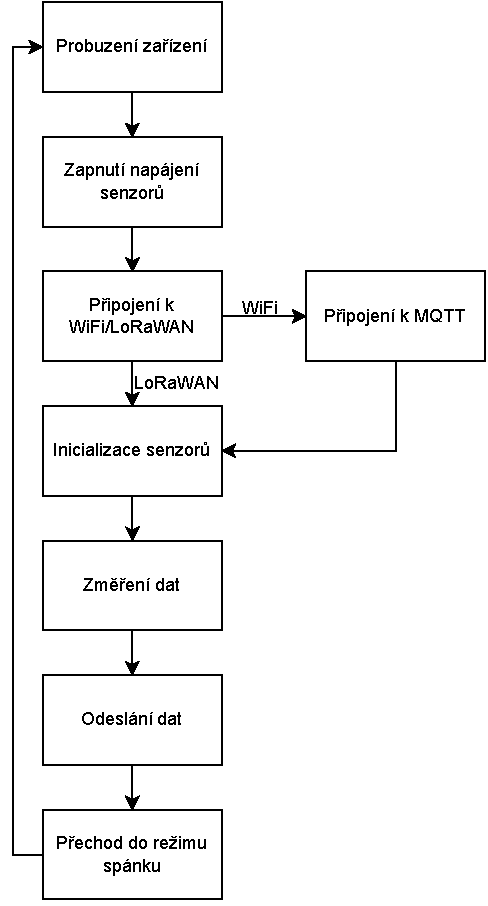
\includegraphics[width=0.4\textwidth]{obrazky/flowchart.pdf}
    \caption{Základní funkce softwaru pro mikrokontroler.}
    \label{fig_flowchart}
\end{figure}

Jak již bylo zmíněno v~předchozích kapitolách, zařízení bude moci zasílat naměřená data pomocí WiFi nebo pomocí LoRaWAN sítě. Obě sítě vyžadují projít procesem připojení, kde u~WiFi zařízení dostane přidělenou IP adresu a~u~LoRaWAN dojde k~vygenerování klíčů, pomocí kterých se poté šifrují a~zasílají zprávy. Zařízení je koncipováno tak, že může být připojeno pouze k~jedné z~těchto sítí a~toto nastavení je definováno pevně ve firmwaru zařízení. 

\section{Firmware mikrokontroleru}

Celý obslužný firmware pro mikrokontroler je naprogamován za použití frameworku ESP-IDF\footnote{\url{https://docs.espressif.com/projects/esp-idf/en/latest/esp32/}} přímo do výrobce čipu ESP32 Espressif. Tento framework obsahuje spou\-sty knihoven pro obsluhu všech periferií a~sběrnic, které čip obsahuje. Programování probíhá buďto v~jazyce C nebo C\texttt{++}. Bylo zapotřebí napsat veškeré knihovny pro obsluhu připojených senzorů. Tyto knihovny využívají prostředky frameworku pro obsluhu hardwarových periferií jednotlivých sběrnic.

Tento framework je postaven na projektu realtime operačního systému pro mikrokontrolery FreeRTOS\footnote{\url{https://www.freertos.org/}} a~umožňuje tak jednoduše spouštět více vláken, časovače, spravovat fronty a~uživatel se o~to nemusí starat. Díky tomuto systému je software rozdělen do několika oddělených vláken, kde se starají o~inicializaci WiFi rozhraní, spojení s~MQTT brokerem, spojení a~obsluhu LoRaWAN sítě, obsluhu senzorů na sběrnici I$^2$C, SPI nebo UART. Díky tomuto rozdělení do jednotlivých vláken je velice snadné zajistit správné časování pro jednotlivé čtení ze senzorů a~je také možné používat blokující funkce pro čekání, jelikož blokováním jednoho vlákna nedojde k~ovlivnění časování vlákna jiného.

\subsection{Obsluha senzorů}

Jak již bylo zmíněno, pro obsluhu všech připojených senzorů jsou použity vlastní knihovny založené na frameworku ESP-IDF. Tyto knihovny obsahují pouze potřebné čtení, inicializace a~případné restarty senzorů. Není obsažena plná funkčnost dle datasheetu výrobce, jelikož pro tuto aplikaci nejsou všechny funkce senzorů potřebné. Senzory jsou rozděleny do skupin podle druhu použité komunikační sběrnice a~je možné je jednotlivě softwarově vypínat, aby byla minimalizována spotřeba celého zařízení. Dále jsou také zajištěny již dříve zmíněné opakované vyčítání ze senzorů pro koncentraci CO$_2$ a~senzoru prachových částic. Po ukončení jednotlivých měření jsou naměřená data uložena do datové struktury k~pozdějšímu odeslání na server. Celý proces začínající probuzením zařízení z~režimu hlubokého spánku, přes změření dat až po odeslání a~uspání trvá zhruba kolem \SI{30}{\second}.

\subsection{Připojení k~WiFi}

Pro použití zařízení s~WiFi sítí je zapotřebí nakonfigurovat ve zdrojovém kódu použití této sítě a~také další potřebné parametry. Konfigurace probíhá v~souboru \texttt{CMakeLists.txt} umístěném v~hlavní složce se zdrojovými kódy.

\begin{lstlisting}[caption={Nastavení spojení pomocí WiFi}]
add_compile_definitions(WIFI)
# add_compile_definitions(LORAWAN)
...

add_compile_definitions(SSID="")
add_compile_definitions(PWD="")
add_compile_definitions(MQTT_BROKER_URL="")
add_compile_definitions(MQTT_PORT=1883)
add_compile_definitions(MQTT_TOPIC="")
\end{lstlisting}

Nastavení probíhá pomocí zakomentování nebo odkomentování jednotlivých řádků konfiguračního souboru. Zakomentování (nepoužití) se provede pomocí znaku '\#' umístěného na začátek daného řádku. Je tedy třeba takto zakomentovat druhý řádek, který definuje použití sítě LoRaWAN a~odkomentovat první s~WiFi sítí.
V této konfiguraci je dále potřeba doplnit SSID (Service Set Identifier) požadované sítě a~její heslo aby bylo možné se připojit. A~dále nastavení spojení s~MQTT brokerem. Zde má uživatel na výběr, jestli použije pouze IP adresu brokeru (typicky v~lokální síti) nebo použije URL (Uniform Resource Locators) pro spojení skrze síť internet na broker mimo lokální síť. Další z~možných nastavení je port MQTT brokeru, který je ve výchozím stavu nastaven na \SI{1883}{}, ale lze jej v~případě potřeby změnit. Posledním nastavením je tzv. topic pro MQTT (kanál pro publikování dat), který musí být unikátní v~rámci jednoho MQTT brokeru, jinak bude docházet ke konfliktům.

\subsection{Připojení k~LoRaWAN}

Konfigurace připojení k~LoRaWAN síti probíhá ve stejném souboru jako WiFi, tedy \texttt{CMakeLists.txt} v~hlavní složce s~firmware. Bude potřeba vygenerovat klíče pro připojení pomocí portálu The Things Network\footnote{\url{https://www.thethingsnetwork.org/}}. Pro využití této sítě je potřeba si na tomto webu vytvořit účet, který je zdarma. Po přihlášení je potřeba přejít do konzole a~zde zvolit záložku aplikace. Pokud uživatel nemá vytvořenou žádnou aplikaci, uvidí pouze tlačítko "\texttt{+} Add application"{} na které je potřeba kliknout a~vytvořit tak novou aplikaci. V~této aplikaci poté budou sdruženy jednotlivá připojená zařízení a~lze na ně aplikovat různé nastavení globálně. Při vytváření aplikace je zapotřebí vyplnit minimálně unikátní id aplikace (bez diakritiky, mezer, \dots), dále je možné vyplnit jméno aplikace, které bude lidsky čitelné a~případný popis aplikace.

\begin{figure}[h]
    \centering
    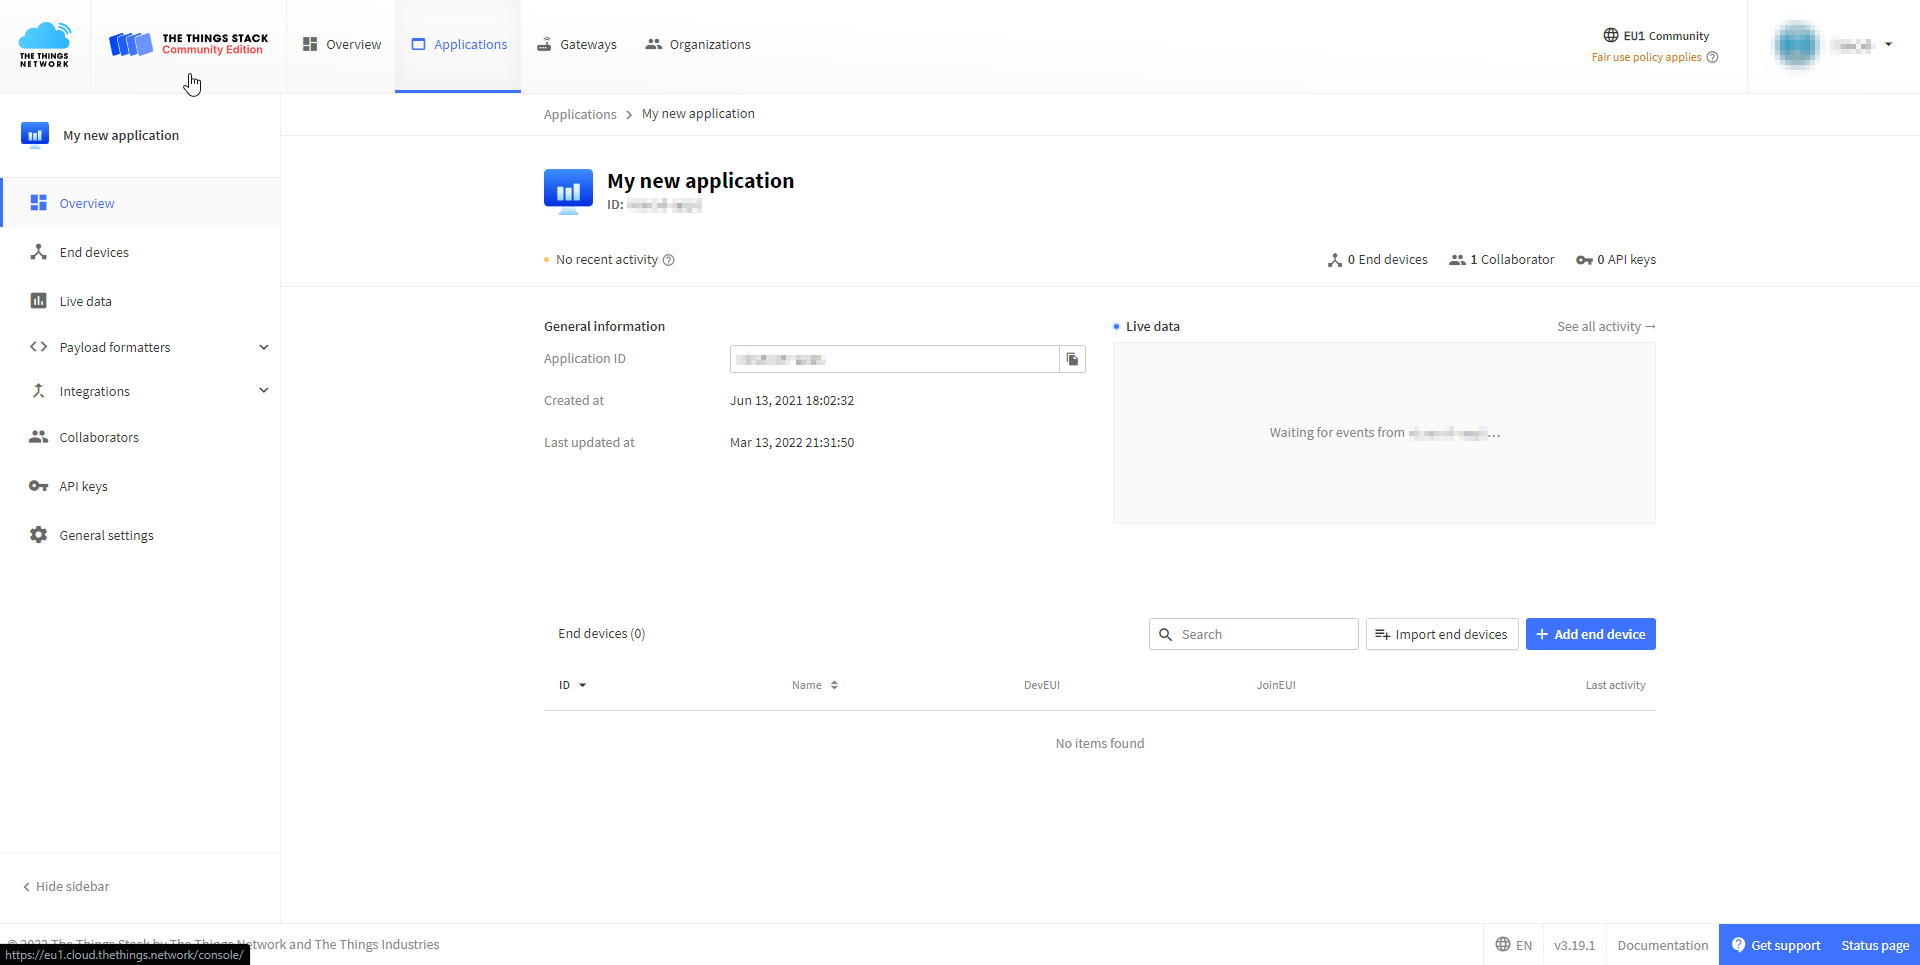
\includegraphics[width=\textwidth]{obrazky/ttnApps.png}
    \caption{Vytvořená aplikace v~konzoli The Things Network.}
    \label{fig_TTNApp}
\end{figure}

Po vytvoření aplikace je možné ji otevřít a~vidět veškeré informace, tak jako na obrázku \ref{fig_TTNApp}. Nyní je potřeba pomocí tlačítka "+ Add end device"{} přidat koncové zařízení a~vytvořit pro něj připojovací unikátní klíče. Některá zařízení schválená službou The Things Network lze přidat automaticky, ale zde je třeba zvolit manuální možnost registrace. Jako první z~nastavení bude třeba zvolit frekvenční plán, pro Evropu je doporučen plán s~názvem "Europe 863-870~MHz (SF9 for RX2 - recommended)", který doporučuji zvolit. Dále je potřeba zvolit specifikaci LoRaWAN standardu, kde použité knihovny pro obsluhu této sítě plně podporují LoRaWAN specifikaci verze 1.0.3. Poslední z~nastavení jsou již zmíněné aktivační klíče pro metodu OTAA (Over The Air Activation), které necháme vygenerovat pomocí serveru. Je tedy třeba vygenerovat "DevEUI", "AppEUI"{} a~"AppKey", k~čemuž slouží tlačítka vedle těchto parametrů. Pole "AppEUI"{} necháme vyplnit nulami. Poslední z~parametrů, který je možné zvolit je "End device ID", který slouží jako jedinečný identifikátor konkrétního zařízení. Lze jej ponechat na automaticky vygenerované hodnotě, která vychází z~DevEUI. Správně navolené a~vygenerované klíče lze vidět na obrázku \ref{fig_TTNDeviceGeneration}. Všechny tyto tři vygenerované unikátní klíče jsou potřeba pro následující nastavení v~rámci firmwaru mikrokontroleru.

\begin{figure}[h]
    \centering
    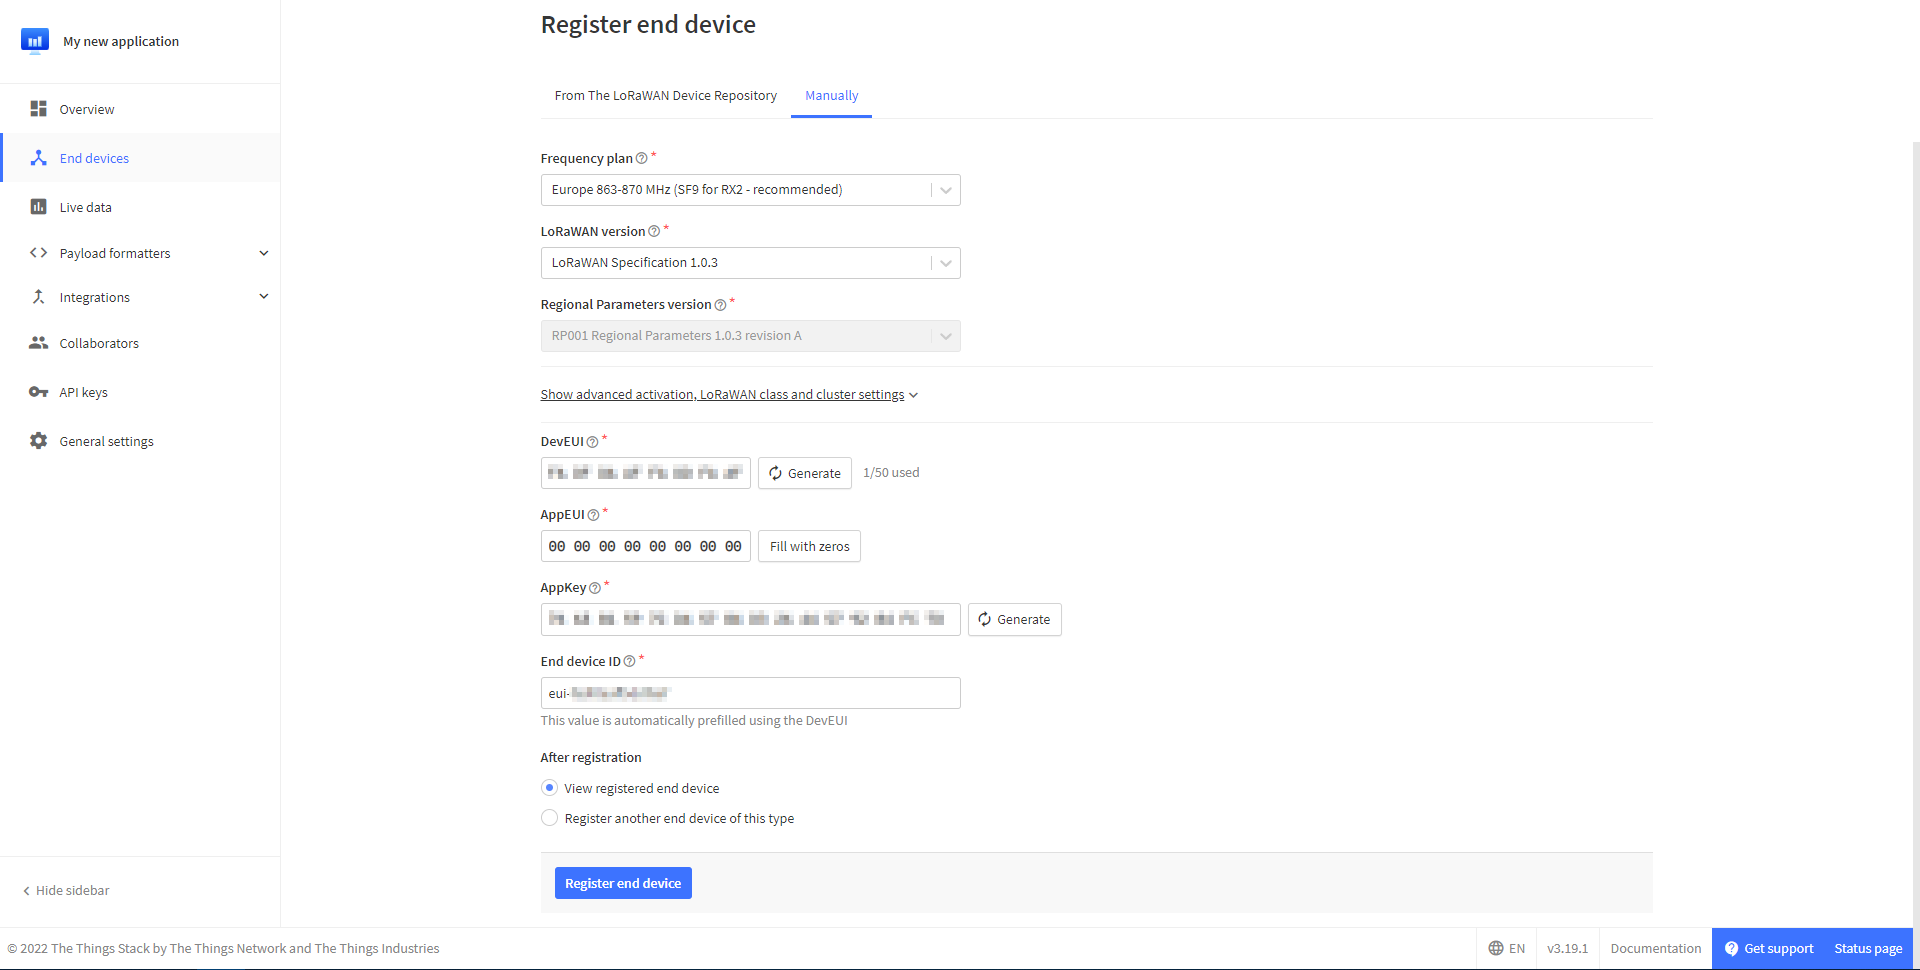
\includegraphics[width=\textwidth]{obrazky/ttnDeviceRegister.png}
    \caption{Formulář pro registraci koncového zařízení do sítě The Things Network.}
    \label{fig_TTNDeviceGeneration}
\end{figure}

V nastavovacím souboru pro firmware je tedy potřeba nastavit zakomentováním řádku s~definicí WiFi a~odkomentováním LoRaWAN použití této sítě. Dále je potřeba do předchystaných definic do uvozovek vložit již zmiňované vygenerované klíče. Při použití této sítě není potřeba nastavovat žádné IP adresy, zprávy se posílají skrze gateway na servery The Things Network, kde se dále zpracovávají.

\begin{lstlisting}[caption={Nastavení spojení pomocí LoRaWAN}]
# add_compile_definitions(WIFI)
add_compile_definitions(LORAWAN)
...

add_compile_definitions(APPEUI="")
add_compile_definitions(DEVEUI="")
add_compile_definitions(APPKEY="")
\end{lstlisting}

\subsection{Frekvence měření}

Poslední z~možností k~nastavení v~rámci firmwaru mikrokontroleru je frekvence měření. Zařízení se spustí, provede měření a~odešle data a~poté je v~režimu hlubokého spánku, kde jsou vypnuty veškeré nepotřebné periferie a~je tak dosahováno co nejnižší spotřeby. Uživatel může nastavení délky tohoto spánku ovlivnit v~souboru \texttt{CMakeLists.txt} pomocí parametru \texttt{SLEEP_TIME}. Tento parametr určuje, jak dlouho bude mikrokontroler v~režimu spánku a~je udáván v~minutách. Pro účely testování používám nastavení \SI{10}{\minute}.

\section{Přijetí dat a~jejich zpracování}

Všechny aplikace pro příjem a~zpracování dat včetně databáze jsou nainstalovány na Raspberry Pi 4. Běží zde tedy Eclipse Mosquitto MQTT broker, Node-RED pro zpracování dat, InfluxDB pro uložení dat a~Grafana pro grafickou vizualizaci dat. Webové rozhraní je dostupné z~lokální sítě, ale lze toto rozhraní zpřístupnit pomocí veřejné IP adresy nebo jiných služeb odkudkoli z~internetu. Zjednodušený diagram procesu přenosu dat je vidět na obrázku \ref{fig_dataFlow}.

\begin{figure}[h]
    \centering
    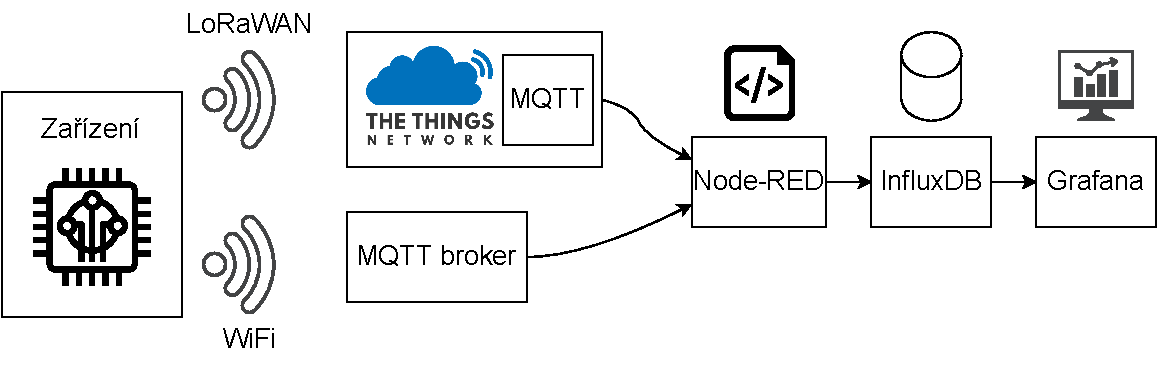
\includegraphics[width=\textwidth]{obrazky/data_flow.pdf}
    \caption{Diagram procesu přenosu dat ze zařízení.}
    \label{fig_dataFlow}
\end{figure}

Naměřená data jsou přímo v~mikrokontroleru naformátována do formátu JSON (JavaScript Object Notation) pro snadné zpracování a~čitelnost. Takovýto přenos dat není z~hlediska přenášeného datového objemu nejefektivnější, ale ani u~WiFi ani u~LoRaWAN nejsme tak striktně omezeni, aby toto řešení nešlo použít. Naměřená data jsou pro zjednodušení programování přenášena jako celá čísla a~na straně serveru je tedy potřeba data převést zpět na desetinná čísla. Ve výpisu \ref{code_JSON} je vidět ukázková JSON struktura, kterou zařízení posílá. Na každém řádku je jedna měřená veličina a~to napětí baterie, hodnota UV záření, teplota, vlhkost, intenzita osvětlení, tlak, prachové částice o~velikosti \SI{1}{\micro\metre}, \SI{2.5}{\micro\metre} a~\SI{10}{\micro\metre}, hodnota koncentrace CO$_2$ a~poslední hodnotou je TVOC. Je nutné mít na paměti, že zde nejsou respektovány veličiny, jelikož jsou čísla přenášená celočíselně.

\noindent
\begin{minipage}{\linewidth}
\begin{lstlisting}[caption={Příklad zasílané JSON zprávy.}, label={code_JSON}]
{
    "B":3334,
    "U":0,
    "T":214,
    "H":437,
    "L":0,
    "P":1013959,
    "P1":27,
    "P25":1,
    "P10":0,
    "C":400,
    "E":0
}
\end{lstlisting}
\end{minipage}

Jak již bylo zmíněno v~předchozích kapitolách, příjem dat na straně serveru je zajištěn MQTT brokerem Eclipse Mosquitto při použití WiFi. MQTT funguje na principu publish-subscribe, což znamená že zařízení se připojí a~publikují svá data do přidělených kanálů odkud mohou ostatní zařízení tato data číst. V~tomto případě má tento topic název podle definice v~konfiguraci firmwaru a~vypadá následovně: \lstinline{air-monitor/zvolený_název/values}. Tento název bude potřeba pro konfiguraci v~Node-RED rozhraní. Pro příjem dat z~portálu The Things Network bude využit jejich MQTT broker ke kterému se připojí Node-RED jako klient a~získá data z~kanálu pro uplink pro jednotlivá připojená zařízení.

\subsection{Konfigurace Node-RED}

Node-RED je nástroj, který umožňuje navzájem spojit zařízení, API aplikací a~provádět jednoduché zpracování dat. Jeho nastavování probíhá skrze webové rozhraní. V~této aplikaci bude zpracovávat přijatá data a~ukládat je do databáze. Pro konfiguraci toku dat slouží tzv. nody, které mají buďto definovanou funkci a~nebo lze vytvořit obecnou funkci v~JavaScriptu.

Konfigurace použitá v~této konkrétní aplikaci je vidět na obrázku \ref{fig_NodeRED}. Jsou zde dvě hlavní větvě, kde horní zpracovává data přenesená přes WiFi z~lokálního MQTT brokeru a~spodní přijímá přes MQTT data z~The Things Network. V~této větvi jsou extrahovány funkcí pouze přijatá data, která se poté převedou na JSON objekt a~jsou dále poslány ke zpracování. Jak již bylo zmíněno, data je nutné převést do desetinné podoby, což se děje v~node s~názvem "Int to float"{} jejíž definici lze vidět na výpisu \ref{code_intToFloat}. Poslední node pouze zapisuje data do předem zvolené tabulky v~InfluxDB databázi.

\begin{figure}[h]
    \centering
    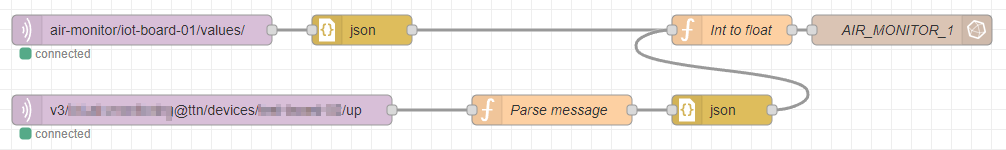
\includegraphics[width=\textwidth]{obrazky/nodered.png}
    \caption{Konfigurace toku dat v~prostředí Node-RED.}
    \label{fig_NodeRED}
\end{figure}

\noindent
\begin{minipage}{\linewidth}
\begin{lstlisting}[caption={Funkce pro převod naměřených dat do desetinné podoby.}, label={code_intToFloat}]
msg.payload = [
    {
        T: (msg.payload["T"] / 10),
        H: (msg.payload["H"] / 10),
        L: msg.payload["L"],
        P: (msg.payload["P"] / 10),
        C: msg.payload["C"],
        E: msg.payload["E"],
        P1: msg.payload["P1"],
        P25: msg.payload["P25"],
        P10: msg.payload["P10"],
        U: (msg.payload["U"] / 1000000),
        B: (msg.payload["B"] / 1000)
    }]
return msg;
\end{lstlisting}
\end{minipage}

\subsection{Grafické uživatelské rozhraní}

O zobrazení dat se stará služba Grafana, která si naměřená data bere přímo z~databáze InfluxDB a~zobrazuje je podle definice uživatele. Je zde mnoho možností na konfiguraci zobrazených prvků jako jsou grafy, bargrafy, status bary, pouze číselné hodnoty a~jiné. Rozložení závisí čistě na uživateli a~jeho preferencích. Zároveň se lze v~již daném rozložení panelů přepínat v~zobrazeném časovém úseku. Služba sama o~sobě umožňuje zobrazit např. posledních \SI{5}{\minute} až několik posledních let a~nebo lze definovat vlastní časový úsek. Dále lze také zapnout automatické obnovování a~mít tak tuto službu v~bezobslužném módu kde bude neustále zobrazovat aktuální data. Příklad takového zobrazení je vidět na obrázku \ref{fig_Grafana}, jsou zde v~grafech vyneseny aktuální hodnoty a~na pravé straně je vidět status bar se stavem baterie a~zároveň pro letmou informaci maximální hodnota teploty za posledních \SI{24}{\hour}.

\begin{figure}[h]
    \centering
    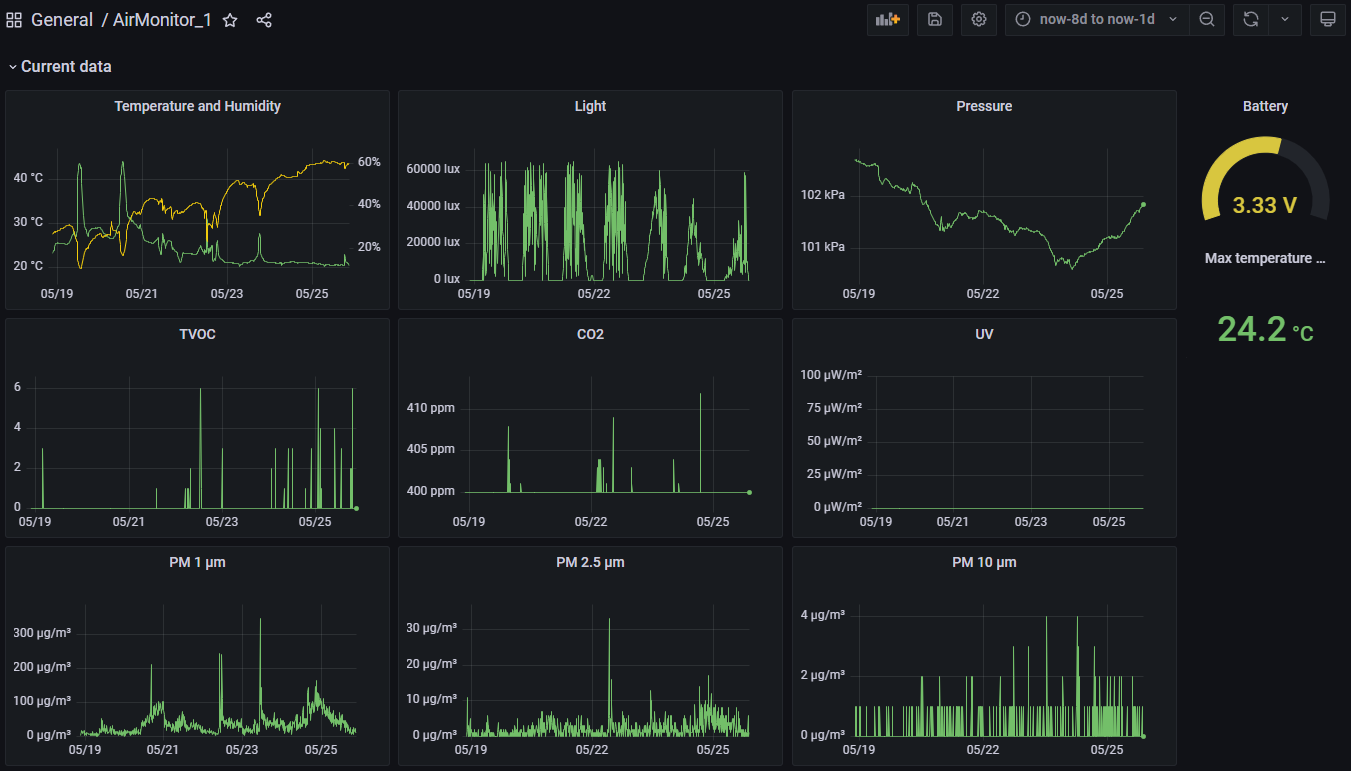
\includegraphics[width=\textwidth]{obrazky/grafana_dark.png}
    \caption{Ukázka zobrazení naměřených dat pomocí aplikace Grafana.}
    \label{fig_GrafanaCurrentData}
\end{figure}

\begin{figure}[h]
    \centering
    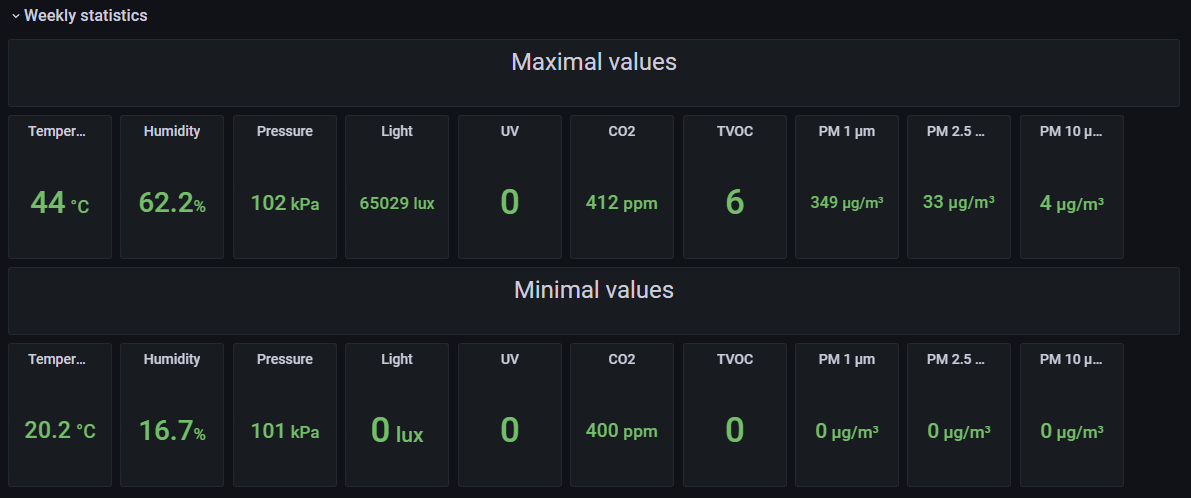
\includegraphics[width=\textwidth]{obrazky/grafana_weeklyStatisticsDark.png}
    \caption{Ukázka zobrazení týdenních maxim a minim pomocí aplikace Grafana.}
    \label{fig_Grafana}
\end{figure}